\documentclass{beamer}
\usepackage[utf8]{inputenc}
\usepackage{listings}
\usepackage{color}
\usepackage{relsize}
\usepackage{graphicx}
\usepackage{array,multirow}
\usepackage{colortbl}

\usetheme{Montpellier}

% code in slides
\newcommand{\code}[1]{\texttt{#1}}
% highlight code in listings
\newcommand{\hili}[1]{\textbf{\color{red} #1}}

\lstset{
 basicstyle=\tiny,
 showspaces=false,
 showstringspaces=false,
 frame=single,
 stringstyle=\ttfamily,
 escapechar=\%,
 columns=space-flexible
}

\title{Spring Batch Workshop (advanced)}
\author{Arnaud Cogoluègnes}
\institute{Consultant with Zenika, Co-author Spring Batch in Action}

\setbeamertemplate{navigation symbols}{}
\logo{
\includegraphics[height=0.5cm]{figures/logo_zenika.png}}
\definecolor{logo}{rgb}{0.58,0.15,0.13}
\definecolor{zenika}{rgb}{0.90,0.91,0.91}
\definecolor{site}{rgb}{0.30,0.30,0.30}
\setbeamercolor{structure}{fg=zenika}
\setbeamercolor{title}{fg=black}
\setbeamercolor{section in head/foot}{fg=logo}
\setbeamercolor{frametitle}{fg=logo}
\setbeamercolor{section in toc}{fg=site}

\begin{document}

\begin{frame}
\titlepage
\end{frame}

\begin{frame}
 \frametitle{Outline}
 \scriptsize{\tableofcontents}
\end{frame}

\section{Overview}

\begin{frame}
\frametitle{Overview}
\begin{itemize}
	\item This workshop highlights advanced Spring Batch features
	\item Problem/solution approach
	\begin{itemize}
		\item A few slides to cover the feature
		\item A project to start from, just follow the TODOs
	\end{itemize}
	\item Prerequisites
	\begin{itemize}
		\item Basics about Java and Java EE
		\item Spring: dependency injection, enterprise support
		\item Spring Batch: what the first workshop covers
	\end{itemize}
	\item https://github.com/acogoluegnes/Spring-Batch-Workshop
\end{itemize}

\end{frame}

\begin{frame}
\frametitle{License}

This work is licensed under the Creative Commons Attribution-NonCommercial-ShareAlike 3.0 
Unported License. 

To view a copy of this license, 
visit http://creativecommons.org/licenses/by-nc-sa/3.0/ or 
send a letter to Creative Commons, 444 Castro Street, Suite 900, Mountain View, 
California, 94041, USA.

\end{frame}

\section{XML file reading}

\begin{frame}
 \begin{itemize}
  \item Problem: reading items from a XML file and sending them to another source (e.g. database)
  \item Solution: using the \code{StaxEventItemReader}
 \end{itemize}
\end{frame}

\begin{frame}
 \frametitle{Spring Batch's support for XML file reading}
 \begin{itemize}
  \item Spring Batch has built-in support for XML files
  \begin{itemize}
    \item Through the \code{StaxEventItemReader} for reading
  \end{itemize}  
  \item The \code{StaxEventItemReader} handles I/O for efficient XML processing
  \item 2 main steps: 
  \begin{itemize}
    \item Configuring the \code{StaxEventItemReader}
    \item Configuring a Spring OXM's \code{Unmarshaller}
  \end{itemize}
 \end{itemize}
\end{frame}

\begin{frame}[fragile]
 \frametitle{The usual suspects}
 \lstset{language=XML}
 \begin{lstlisting}
<?xml version="1.0" encoding="UTF-8"?>
<contacts>
  <contact>
    <firstname>De-Anna</firstname>
    <lastname>Raghunath</lastname>
    <birth>2010-03-04</birth>
  </contact>
  <contact>
    <firstname>Susy</firstname>
    <lastname>Hauerstock</lastname>
    <birth>2010-03-04</birth>
  </contact>
  (...)
</contacts>
\end{lstlisting}

\begin{center}
\begin{picture}(0,0)
\put(0,15){\vector(0,-1){15}} 
\end{picture}
\end{center}

\lstset{language=Java}
\begin{lstlisting}
public class Contact {

  private Long id;
  private String firstname,lastname;
  private Date birth;
  
  (...)
}
\end{lstlisting}

\end{frame}

\begin{frame}[fragile]
 \frametitle{The \code{StaxEventItemReader} configuration}

\lstset{language=XML}
\begin{lstlisting}
<bean id="reader" class="org.springframework.batch.item.xml.StaxEventItemReader">
  <property name="fragmentRootElementName" value="contact" />
  <property name="unmarshaller">
    <bean class="org.springframework.oxm.xstream.XStreamMarshaller">
      <property name="aliases">
        <map>
          <entry key="contact" value="com.zenika.workshop.springbatch.Contact" />
        </map>
      </property>
      <property name="converters">
        <bean class="com.thoughtworks.xstream.converters.basic.DateConverter">
          <constructor-arg value="yyyy-MM-dd" />
          <constructor-arg><array /></constructor-arg>
          <constructor-arg value="true" />
        </bean>
      </property>
    </bean>
  </property>
  <property name="resource" value="classpath:contacts.xml" />
</bean>
\end{lstlisting}
  \begin{itemize}
    \item NB: Spring OXM supports XStream, JAXB2, etc. 
  \end{itemize}
\end{frame}

\begin{frame}
 \frametitle{Going further...}
 \begin{itemize}
  \item \code{StaxEventItemWriter} to write XML files
  \item Spring OXM's support for other marshallers
  \item Skipping badly formatted lines
 \end{itemize}
\end{frame}
\section{Item enrichment}

\begin{frame}
 \begin{itemize}
  \item Problem: I want to enrich read items with a Web Service before they get written
  \item Solution: implement an \code{ItemProcessor} to make the Web Service call
 \end{itemize}
\end{frame}

\begin{frame}
 \frametitle{Use case}
 \begin{itemize}
  \item Reading contacts from a flat file
  \item Enriching the contact with their social security number  
  \item Writing the whole contact in the database
 \end{itemize}
\end{frame}


\begin{frame}[fragile]
\begin{textcode}
1,De-Anna,Raghunath,2010-03-04
2,Susy,Hauerstock,2010-03-04
3,Kiam,Whitehurst,2010-03-04
4,Alecia,Van Holst,2010-03-04
5,Hing,Senecal,2010-03-04
\end{textcode}
\begin{itemize}
 \item NB: no SSN in the CSV file!
\end{itemize}
\begin{javacode}
public class Contact {

  private Long id;	
  private String firstname,lastname;	
  private Date birth;	
  private String ssn;
  (...)
}
\end{javacode}
\end{frame}

\begin{frame}[fragile]
\frametitle{The Web Service}
\begin{itemize}
 \item It can be any kind of Web Service (SOAP, REST)
 \item Our Web Service
 \begin{itemize}
    \item URL: \code{http://host/service?firstname=John\&lastname=Doe}
    \item It returns
 \end{itemize} 
\end{itemize}

\begin{xmlcode}
<contact>
  <firstname>John</firstname>
  <lastname>Doe</lastname>
  <ssn>987-65-4329</ssn>
</contact>
\end{xmlcode}
\end{frame}

\begin{frame}[fragile]
\frametitle{The \code{ItemProcessor} implementation}
\begin{javacode*}{fontsize=\tiny}
package com.zenika.workshop.springbatch;

import javax.xml.transform.dom.DOMSource;
import org.springframework.batch.item.ItemProcessor;
import org.springframework.web.client.RestTemplate;
import org.w3c.dom.NodeList;

public class SsnWebServiceItemProcessor implements
             ItemProcessor<Contact, Contact> {
	
  private RestTemplate restTemplate = new RestTemplate();
  private String url;

  @Override
  public Contact process(Contact item) throws Exception {
    DOMSource source = restTemplate.getForObject(url,DOMSource.class, 
      item.getFirstname(),item.getLastname());
    String ssn = extractSsnFromXml(item, source);
    item.setSsn(ssn);
    return item;
  }

  private String extractSsnFromXml(Contact item, DOMSource source) {
    // some DOM code
  }
  (...)
}
\end{javacode*}
\end{frame}

\begin{frame}[fragile]
\frametitle{Configuring the \code{SsnWebServiceItemProcessor}}
\begin{xmlcode*}{fontsize=\tiny}
<batch:job id="itemEnrichmentJob">
  <batch:step id="itemEnrichmentStep">
    <batch:tasklet>
      <batch:chunk reader="reader" processor="processor" writer="writer" 
                   commit-interval="3"/>
    </batch:tasklet>
  </batch:step>
</batch:job>

<bean id="processor" 
      class="com.zenika.workshop.springbatch.SsnWebServiceItemProcessor">
  <property name="url" 
  value="http://localhost:8085/?firstname={firstname}&amp;lastname={lastname}" />
</bean>
\end{xmlcode*}
\end{frame}

\begin{frame}
 \frametitle{But my Web Service has a lot of latency!}
 \begin{itemize}
  \item The Web Service call can benefit from multi-threading
  \item Why not spawning several processing at the same time?
  \item We could wait for the completion in the \code{ItemWriter}
  \item Let's use some asynchronous \code{ItemProcessor} and \code{ItemWriter}
  \begin{itemize}
    \item Provided in the Spring Batch Integration project
  \end{itemize}  
 \end{itemize}
\end{frame}

\begin{frame}[fragile]
\frametitle{Using async \code{ItemProcessor} and \code{ItemWriter}}
\begin{itemize}
  \item This is only about wrapping  
 \end{itemize}
\begin{xmlcode}
<bean id="processor"
      class="o.s.b.integration.async.AsyncItemProcessor">
  <property name="delegate" ref="processor" />
  <property name="taskExecutor" ref="taskExecutor" />
</bean>

<bean id="writer"
      class="o.s.b.integration.async.AsyncItemWriter">
  <property name="delegate" ref="writer" />							
</bean>

<task:executor id="taskExecutor" pool-size="5" />
\end{xmlcode}
\end{frame}

\begin{frame}
 \frametitle{Going further...}
 \begin{itemize}
  \item Business delegation with an \code{ItemProcessor}
  \item Available \code{ItemProcessor} implementations
  \begin{itemize}
    \item Adapter, validator
  \end{itemize}
  \item The \code{ItemProcessor} can filter items
 \end{itemize}
\end{frame}


\section{File reading partitioning}

\begin{frame}
 \begin{itemize}
  \item Problem: I have multiple input files and I want to process them in parallel
  \item Solution: use partitioning to parallelize the processing on multiple threads
 \end{itemize}
\end{frame}

\begin{frame}
 \frametitle{Serial processing}
 \begin{center}
 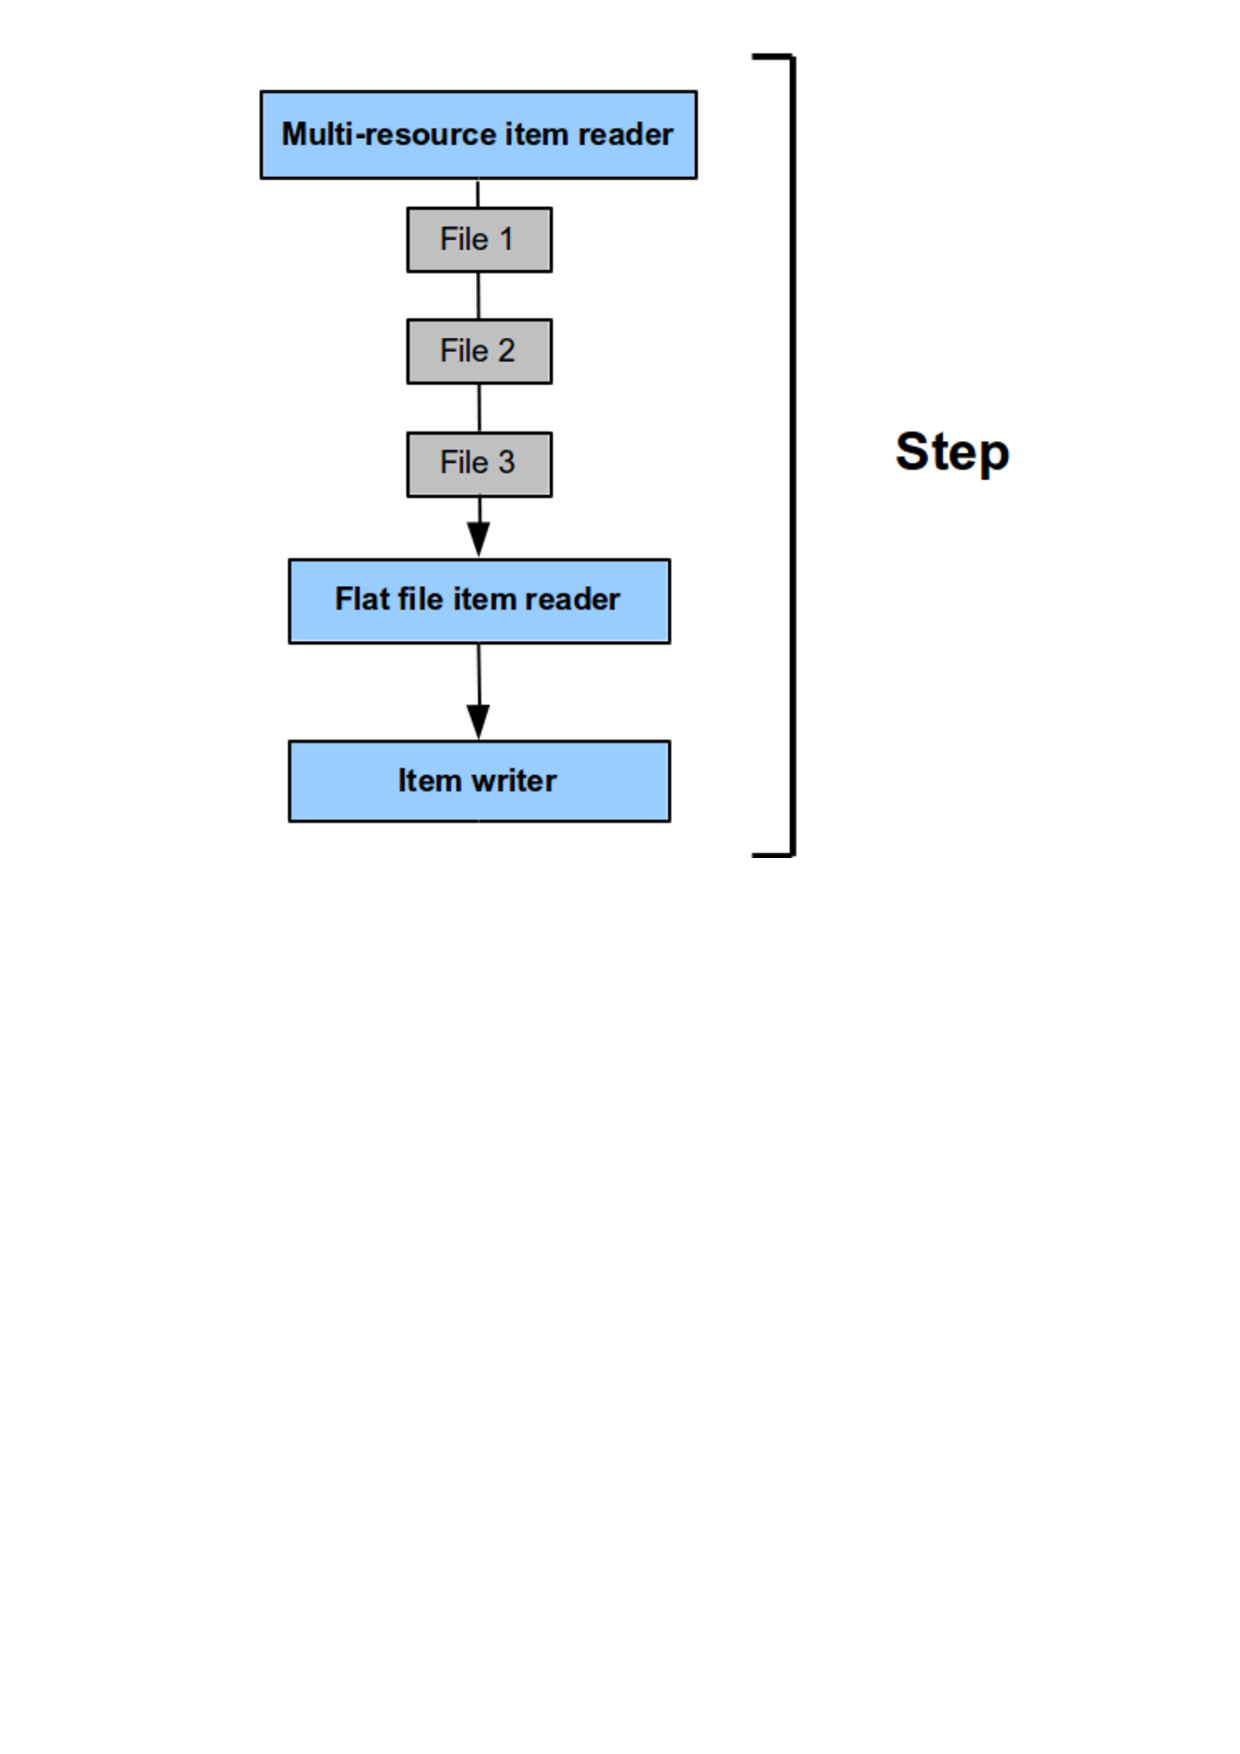
\includegraphics[width=10cm]{figures/input-files-serial.pdf}
 \end{center}
\end{frame}


\begin{frame}
 \frametitle{Partitioning in Spring Batch}
 \begin{itemize}
  \item Partition the input data
  \begin{itemize}
    \item e.g. one input file = one partition
    \item partition processed in a dedicated step execution
  \end{itemize}
  \item Partitioning is easy to set up but need some knowledge about the data
  \item Partition handler implementation
  \begin{itemize}
   \item Multi-threaded
   \item Spring Integration  
  \end{itemize}
 \end{itemize}
\end{frame}

\begin{frame}
 \frametitle{Multi-threaded partitioning}
 \begin{center}
  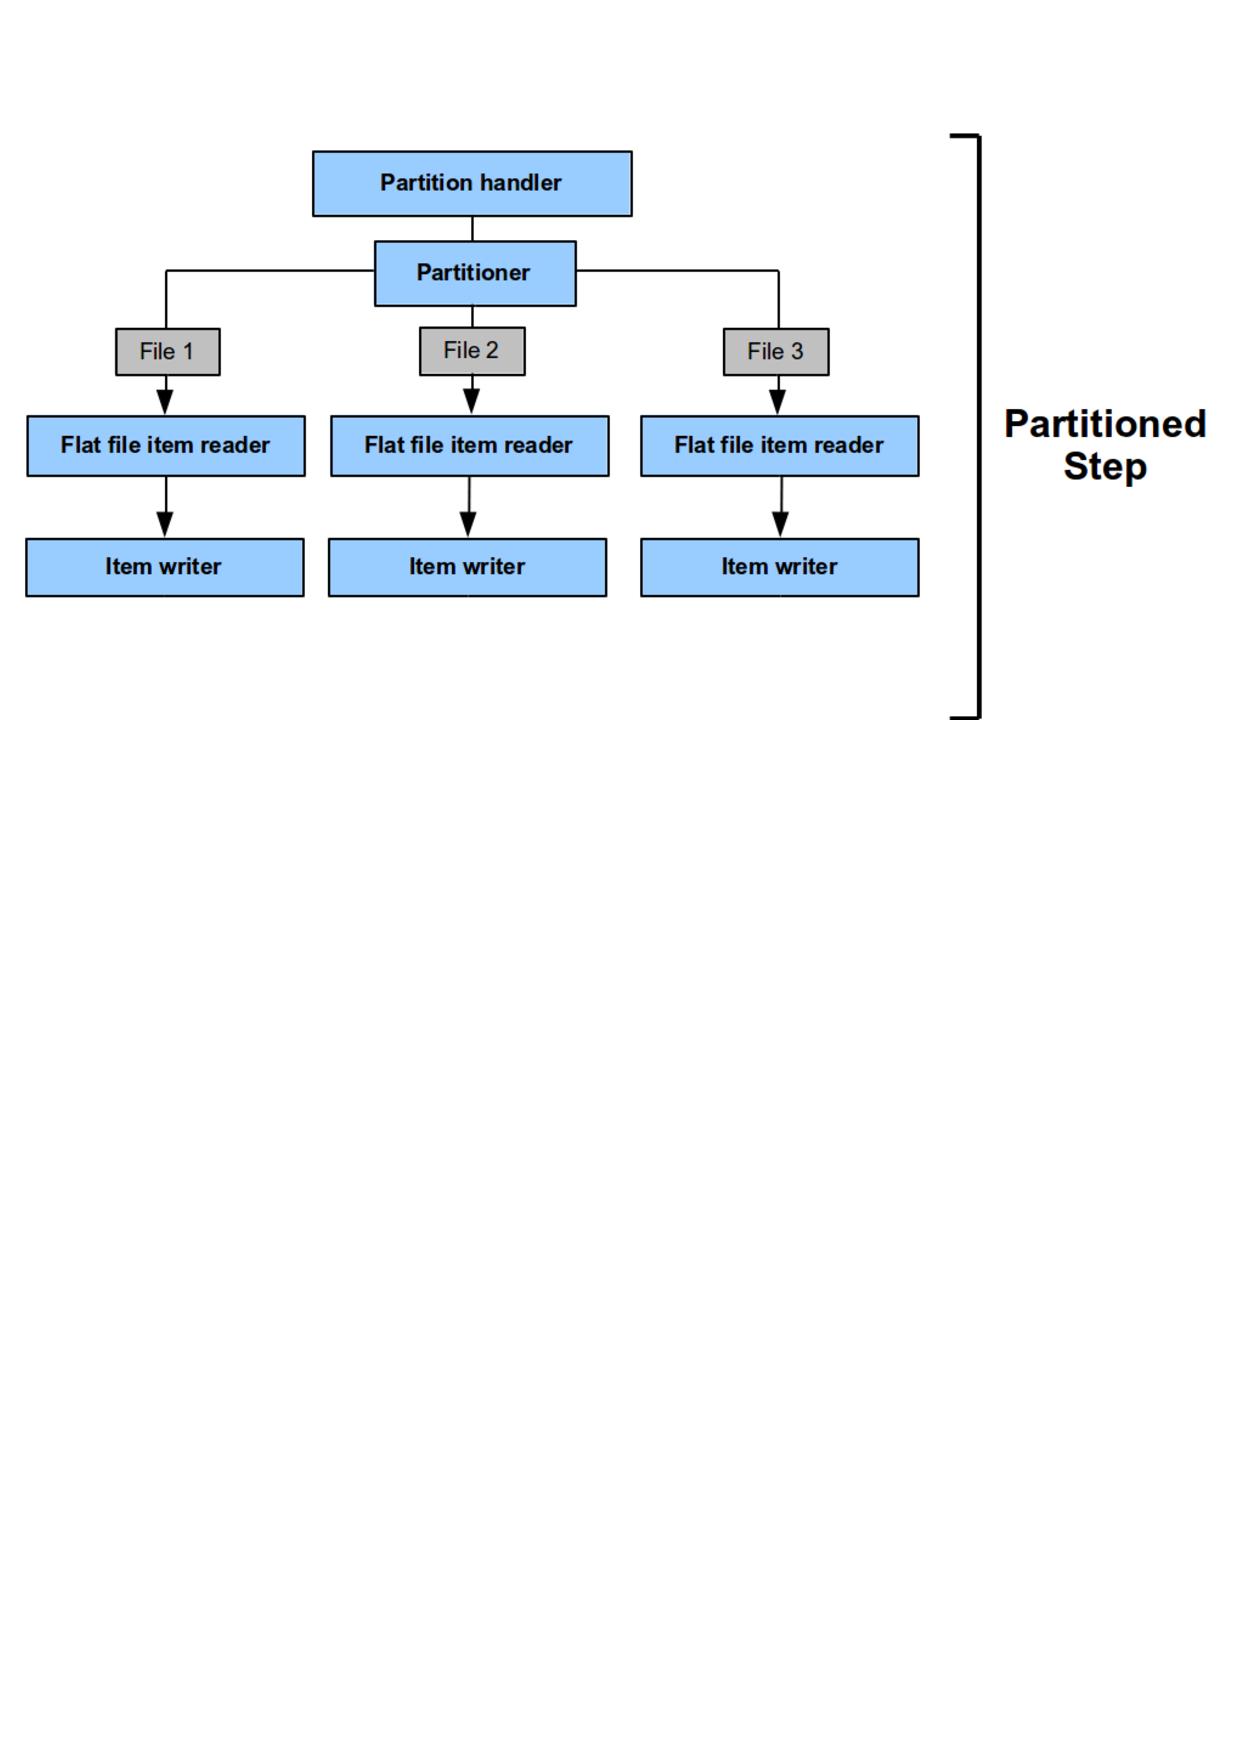
\includegraphics[width=10cm]{figures/input-files-partitioning.pdf}  
 \end{center}
\end{frame}

\begin{frame}[fragile]
\frametitle{Partitioner for input files}
\begin{xmlcode}
<bean id="partitioner"
      class="o.s.b.core.partition.support.MultiResourcePartitioner">
  <property name="resources" 
            value="file:./src/main/resources/input/*.txt" />
</bean>
\end{xmlcode}
\end{frame}

\begin{frame}[fragile]
\frametitle{The partitioner sets a context for the components}

\begin{xmlcode}
<bean id="reader" 
      class="org.springframework.batch.item.file.FlatFileItemReader" 
      scope="step">
  (...)
  <property name="resource" 
            value="#{stepExecutionContext['fileName']}" />
</bean>
\end{xmlcode}
\end{frame}

\begin{frame}[fragile]
 \frametitle{Using the multi-threaded partition handler}
 \begin{xmlcode}
<batch:job id="fileReadingPartitioningJob">
  <batch:step id="partitionedStep" >
    <batch:partition step="readWriteContactsPartitionedStep"
                     partitioner="partitioner">
      <batch:handler task-executor="taskExecutor" />
    </batch:partition>
  </batch:step>
</batch:job>

<batch:step id="readWriteContactsPartitionedStep">
  <batch:tasklet>    
    <batch:chunk reader="reader" writer="writer" 
                 commit-interval="10" />
  </batch:tasklet>	
</batch:step>
 \end{xmlcode}
\end{frame}

\begin{frame}
 \frametitle{Going further...}
 \begin{itemize}
  \item Spring Integration partition handler implementation
  \item Other scaling approaches
  \begin{itemize}
   \item parallel steps, remote chunking, multi-threaded step)
  \end{itemize}  
 \end{itemize}
\end{frame}


\section{File dropping launching}

\begin{frame}
 \begin{itemize}
  \item Problem: downloading files from a FTP server and processing them with Spring Batch
  \item Solution: use Spring Integration to poll the FTP server and trigger Spring Batch accordingly
 \end{itemize}
\end{frame}

\begin{frame}
 \frametitle{Using Spring Integration for transfer and triggering}
 \begin{center}
  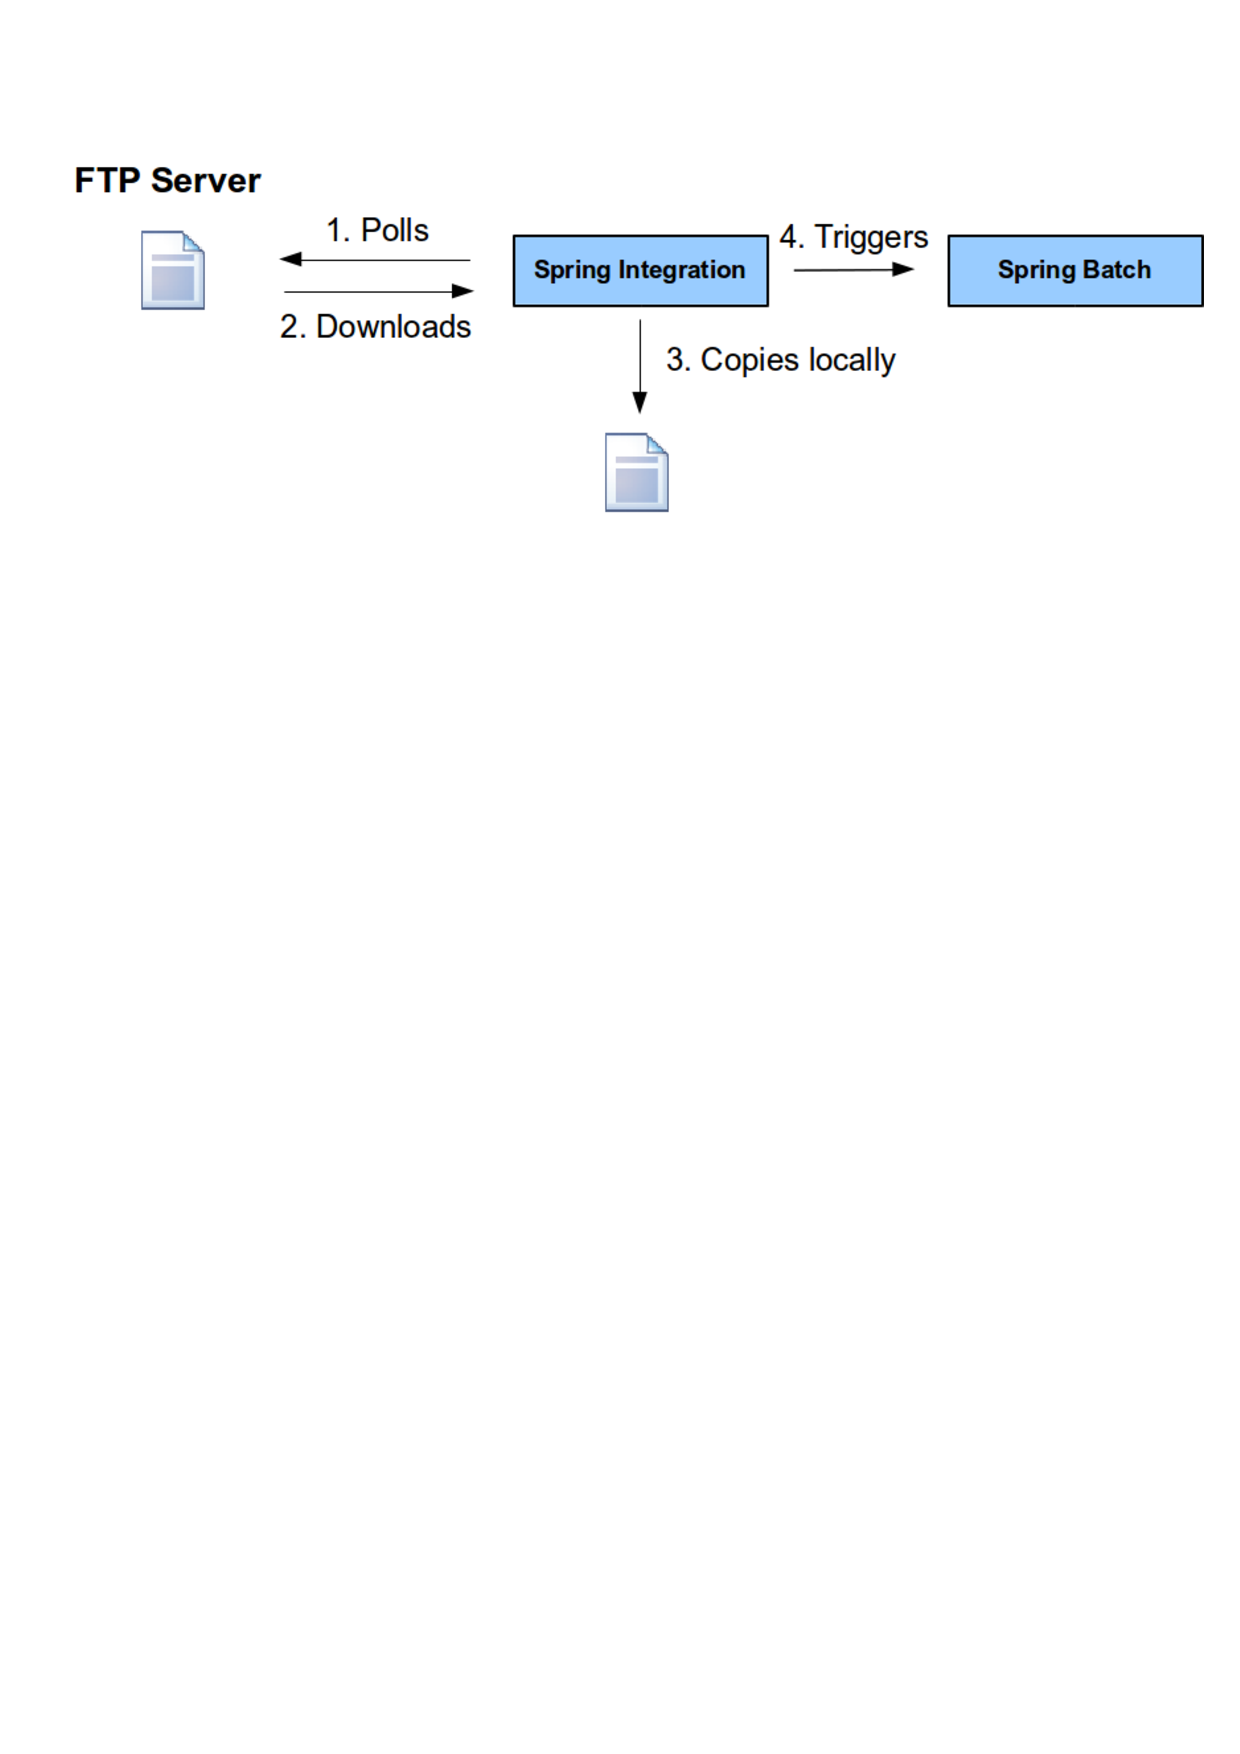
\includegraphics[width=10cm]{figures/spring-integration-ftp-poller.pdf}
 \end{center}
\end{frame}


\begin{frame}[fragile]
 \frametitle{The launching code}
 \lstset{language=Java}
 \begin{lstlisting}
public class FileContactJobLauncher {

  public void launch(File file) throws Exception {
      JobExecution exec = jobLauncher.run(
        job, 
        new JobParametersBuilder()
          .addString("input.file", "file:"+file.getAbsolutePath())
          .toJobParameters()
      );
  }

}  
 \end{lstlisting}

 \begin{itemize}
  \item The \code{File} is the local copy
 \end{itemize}
\end{frame}


\begin{frame}[fragile]
 \frametitle{Listening to the FTP server}
 \lstset{language=XML}
 \begin{lstlisting}
<int:channel id="fileIn" />

<int-ftp:inbound-channel-adapter local-directory="file:./input" 
    channel="fileIn" session-factory="ftpClientFactory" 
    remote-directory="/" auto-create-local-directory="true">
  <int:poller fixed-rate="1000" />
</int-ftp:inbound-channel-adapter>

<bean id="ftpClientFactory"
      class="com.zenika.workshop.springbatch.integration.DefaultFtpSessionFactory">
  <property name="host" value="localhost"/>
  <property name="port" value="2222"/>
  <property name="username" value="admin"/>
  <property name="password" value="admin"/>
</bean>
 \end{lstlisting}
\end{frame}

\begin{frame}[fragile]
\frametitle{Calling the launcher on an inbound message}
\lstset{language=XML}
\begin{lstlisting}
<int:channel id="fileIn" />

<int:service-activator input-channel="fileIn">
  <bean 
    class="com.zenika.workshop.springbatch.integration.FileContactJobLauncher">
    <property name="job" ref="fileDroppingLaunchingJob" />
    <property name="jobLauncher" ref="jobLauncher" />
  </bean>
</int:service-activator>
 \end{lstlisting}
\end{frame}

\begin{frame}
 \frametitle{Going further...}
 \begin{itemize}
  \item Checking Spring Integration connectors
  \begin{itemize}
   \item Local file system, FTPS, SFTP, HTTP, JMS, etc.
  \end{itemize}
  \item Checking operations on messages
  \begin{itemize}
   \item Filtering, transforming, routing, etc.
  \end{itemize}
 \end{itemize}
\end{frame}


\section{Database reading partitioning}

\begin{frame}
 \begin{itemize}
  \item Problem: I want to export items from different categories from a database to files
  \item Solution: provide a partition strategy and use partitioning
 \end{itemize}
\end{frame}

\begin{frame}
 \frametitle{The use case}
 \begin{center}
 \begin{tabular}{l|l|l}
  \hline
  ID & name & category \\
  \hline
  1 & Book 01 & books \\
  2 & DVD 01 & dvds \\
  3 & DVD 02 & dvds \\
  4 & Book 02 & books \\
  \hline
 \end{tabular}
 \end{center}
 \begin{center}
  \begin{picture}(100,0)
   \put(50,0){\line(0,-1){10}}
   \put(0,-10){\line(1,0){100}}
   \put(0,-10){\vector(0,-1){10}}
   \put(100,-10){\vector(0,-1){10}}
  \end{picture}
 \end{center} 
 \begin{center}
  \begin{picture}(150,80)
   % books file
   \put(1,63){\tiny{products\_books.txt}}
   \put(0,0){\line(0,1){60}}
   \put(50,0){\line(0,1){60}}
   \put(0,0){\line(1,0){50}}
   \put(0,60){\line(1,0){50}}
   \put(1,53){\tiny{1,Book 01,books}}
   \put(1,43){\tiny{4,Book 02,books}}
   % dvds file
   \put(101,63){\tiny{products\_dvds.txt}}
   \put(100,0){\line(0,1){60}}
   \put(150,0){\line(0,1){60}}
   \put(100,0){\line(1,0){50}}
   \put(100,60){\line(1,0){50}}
   \put(101,53){\tiny{2,DVD 01,dvds}}
   \put(101,43){\tiny{3,DVD 02,dvds}}   
  \end{picture}
 \end{center}
\end{frame}


\begin{frame}
 \frametitle{Partitioning based on categories}
 \begin{itemize}
  \item 2 partitions in this case  
 \end{itemize}
 \begin{center}
 \begin{tabular}{l|l|l}
  \hline
  ID & name & category \\
  \hline
  \rowcolor{cyan}1 & Book 01 & books \\
  \rowcolor{yellow}2 & DVD 01 & dvds \\
  \rowcolor{yellow}3 & DVD 02 & dvds \\
  \rowcolor{cyan}4 & Book 02 & books \\
  \hline
 \end{tabular}
 \end{center}
\end{frame}


\begin{frame}[fragile]
\frametitle{Partitioning logic with the \code{Partitioner} interface}
\lstset{language=Java}
\begin{lstlisting}
public class ProductCategoryPartitioner implements Partitioner {
  (...)

  @Override
  public Map<String, ExecutionContext> partition(int gridSize) {
    List<String> categories = jdbcTemplate.queryForList(
      "select distinct(category) from product",
      String.class
    );
    Map<String, ExecutionContext> results = 
      new LinkedHashMap<String, ExecutionContext>();
    for(String category : categories) {
      ExecutionContext context = new ExecutionContext();
      context.put("category", category);
      results.put("partition."+category, context);
    } 
    return results;
  }
}
\end{lstlisting}

\end{frame}

\begin{frame}[fragile]
\frametitle{Output of the \code{Partitioner}}

\begin{itemize}
 \item Excerpt: 
\end{itemize}

\lstset{language=Java}
\begin{lstlisting}
for(String category : categories) {
  ExecutionContext context = new ExecutionContext();
  context.put("category", category);
  results.put("partition."+category, context);
}
\end{lstlisting}
\begin{itemize}
 \item Results: 
\end{itemize}

\begin{lstlisting}
partition.books = { category => 'books' }
partition.dvds  = { category => 'dvds' }
\end{lstlisting}

\end{frame}

\begin{frame}[fragile]
\frametitle{Components can refer to partition parameters}
\begin{itemize}
 \item They need to use the step scope 
\end{itemize}

\lstset{language=XML}
\begin{lstlisting}
<bean id="reader" 
      class="org.springframework.batch.item.database.JdbcCursorItemReader" 
      scope="step">
  <property name="sql" 
            value="select id,name,category from product where category = ?" />
  <property name="preparedStatementSetter">
    <bean class="org.springframework.jdbc.core.ArgPreparedStatementSetter">
      <constructor-arg value="%\hili{\#\{stepExecutionContext['category']\}]}%" />
    </bean>
  </property>
</bean>

<bean id="writer" 
      class="org.springframework.batch.item.file.FlatFileItemWriter" 
      scope="step">
  <property name="resource"
     value="%\hili{file:./target/products\_\#\{stepExecutionContext['category']\}.txt}%" />
 
  (...)
</bean>
\end{lstlisting}
\end{frame}

\begin{frame}[fragile]
\frametitle{Configure the partitioned step}
\begin{itemize}
 \item The default implementation is multi-threaded
\end{itemize}

\lstset{language=XML}
\begin{lstlisting}
<batch:job id="databaseReadingPartitioningJob">
  <batch:step id="partitionedStep" >
    <batch:partition step="readWriteProductsPartitionedStep" 
                     partitioner="partitioner">
      <batch:handler task-executor="taskExecutor" />
    </batch:partition>
  </batch:step>
</batch:job>

<batch:step id="readWriteProductsPartitionedStep">
  <batch:tasklet>
    <batch:chunk reader="reader" writer="writer" commit-interval="10" />
  </batch:tasklet>	
</batch:step>
\end{lstlisting}
\end{frame}

\begin{frame}
 \frametitle{Going further...}
 \begin{itemize}
  \item Check existing partitioner implementations
  \item Check other partition handler implementations
  \item Check other scaling strategies
 \end{itemize}
\end{frame}


\section{Complex flow}

\begin{frame}
 \begin{itemize}
  \item Problem: my job has a complex flow of steps, how can Spring Batch deal with it?
  \item Solution: use the step flow attributes and tags, as well as \code{StepExecutionListener}s.
 \end{itemize}
\end{frame}

\begin{frame}[fragile]
 \frametitle{The \code{next} attribute for a linear flow}
 \lstset{language=XML}
\begin{lstlisting}
<batch:job id="complexFlowJob">
  <batch:step id="digestStep" next="%\hili{flatFileReadingStep}%">
    <batch:tasklet ref="digestTasklet" />
  </batch:step>		
  <batch:step id="%\hili{flatFileReadingStep}%">
    <batch:tasklet>
      <batch:chunk reader="reader" writer="writer" commit-interval="3" />
    </batch:tasklet>		
  </batch:step>	
</batch:job>
\end{lstlisting}
\end{frame}

\begin{frame}[fragile]
 \frametitle{There's also a \code{next} tag non-linear flows}
 \lstset{language=XML}
\begin{lstlisting}
<batch:job id="complexFlowJob">
  <batch:step id="digestStep">
    <batch:tasklet ref="digestTasklet" />
    <batch:next on="COMPLETED" to="%\hili{flatFileReadingStep}%"/>
    <batch:next on="FAILED" to="%\hili{trackIncorrectFileStep}%"/>
  </batch:step>
  <batch:step id="%\hili{flatFileReadingStep}%">
    <batch:tasklet>
      <batch:chunk reader="reader" writer="writer" commit-interval="3" />
    </batch:tasklet>
  </batch:step>
  <batch:step id="%\hili{trackIncorrectFileStep}%">
    <batch:tasklet ref="trackIncorrectFileTasklet" />
  </batch:step>
</batch:job>
\end{lstlisting}
\begin{itemize}
 \item NB: there are also the \code{end}, \code{fail}, and \code{stop} tags
\end{itemize}

\end{frame}

\begin{frame}
 \frametitle{But if I have more complex flows?}
 \begin{itemize}
  \item The \code{next} attribute decision is based on the exit code
  \item You can use your own exit codes
  \item A \code{StepExecutionListener} can modify the exit code of a step execution
 \end{itemize}

\end{frame}

\begin{frame}[fragile]
 \frametitle{Modifying the exit code of a step execution}
 \lstset{language=Java}
 \begin{lstlisting}
package com.zenika.workshop.springbatch;

import org.springframework.batch.core.ExitStatus;
import org.springframework.batch.core.StepExecution;
import org.springframework.batch.core.StepExecutionListener;

public class SkipsListener implements StepExecutionListener {

  @Override
  public void beforeStep(StepExecution stepExecution) { }

  @Override
  public ExitStatus afterStep(StepExecution stepExecution) {
    String exitCode = stepExecution.getExitStatus().getExitCode();
    if (!exitCode.equals(ExitStatus.FAILED.getExitCode()) && 
              stepExecution.getSkipCount() > 0) {
      return new ExitStatus("COMPLETED WITH SKIPS");
    } else {
      return null;
    }
  }
}
\end{lstlisting}

\end{frame}


\begin{frame}[fragile]
 \frametitle{Plugging the \code{SkipsListener}}

\lstset{language=XML}
\begin{lstlisting}
<step id="flatFileReadingStep">
  <tasklet>
    <chunk reader="reader" writer="writer" 
           commit-interval="3" skip-limit="10">
      <skippable-exception-classes>
        <include 
        class="org.springframework.batch.item.file.FlatFileParseException"/>
      </skippable-exception-classes>
    </chunk>
  </tasklet>		
  <end on="COMPLETED"/>	
  %\hili{\textless next on="COMPLETED WITH SKIPS" to="trackSkipsStep"/\textgreater}%
  <listeners>
    <listener>
      %\hili{\textless beans:bean class="com.zenika.workshop.springbatch.SkipsListener" /\textgreater}%
    </listener>
  </listeners>
</step>
\end{lstlisting}

\end{frame}

\begin{frame}
 \frametitle{Going further...}
 \begin{itemize}
  \item The \code{JobExecutionDecider} and the \code{decision} tag
  \item The \code{stop}, \code{fail}, and \code{end} tags
 \end{itemize}
\end{frame}
\section{Atomic processing}

\begin{frame}
 \begin{itemize}
  \item Problem: I want to process an input file in an all-or-nothing manner.
  \item Solution: Don't do it. Atomic processing isn't batch processing! Anyway, if you really need 
  an atomic processing, use a custom \code{CompletionPolicy}.
 \end{itemize}
\end{frame}

\begin{frame}
 \frametitle{Why atomic processing is a bad idea?}
 \begin{itemize}
  \item You loose the benefits of chunk-oriented processing
  \begin{itemize}
    \item speed, small memory footprint, etc.
  \end{itemize}
  \item On a rollback, you loose everything (that's perhaps the point!)
  \item The rollback can take a long time (several hours)
  \item It all depends on the amount of data and on the processing
 \end{itemize}
\end{frame}

\begin{frame}
 \frametitle{I really need an atomic processing}
 \begin{itemize}
  \item Rollback yourself, with compensating transactions  
  \item Use a transaction rollback
  \begin{itemize}
    \item It's only a never ending chunk!
  \end{itemize}
 \end{itemize}
\end{frame}

\begin{frame}[fragile]
 \frametitle{Quick and dirty, large commit interval}
 \begin{itemize}
  \item Set the commit interval to a very large value  
  \item You should never have more items!
 \end{itemize}
 \lstset{language=XML}
\begin{lstlisting}
<batch:chunk reader="reader" writer="writer" commit-interval="1000000"/>
\end{lstlisting}
\end{frame}

\begin{frame}[fragile]
 \frametitle{Use a never-ending \code{CompletionPolicy}}
 \begin{itemize}
  \item Spring Batch uses a \code{CompletionPolicy} to know if a chunk is complete
 \end{itemize}
 \lstset{language=Java}
\begin{lstlisting}
package org.springframework.batch.repeat;

public interface CompletionPolicy {

  boolean isComplete(RepeatContext context, RepeatStatus result);

  boolean isComplete(RepeatContext context);

  RepeatContext start(RepeatContext parent);

  void update(RepeatContext context);

}
\end{lstlisting}
\end{frame}

\begin{frame}[fragile]
 \frametitle{Plugging in the \code{CompletionPolicy}}
 \lstset{language=XML}
\begin{lstlisting}
<batch:job id="atomicProcessingJob">
  <batch:step id="atomicProcessingStep">
    <batch:tasklet>
      <batch:chunk reader="reader" writer="writer" 
                   %\hili{chunk-completion-policy="atomicCompletionPolicy"}% />
    </batch:tasklet>
  </batch:step>
</batch:job>
\end{lstlisting}
\begin{itemize}
  \item NB: remove the \code{commit-interval} attribute when using a \code{CompletionStrategy}
 \end{itemize}
\end{frame}

\begin{frame}[fragile]
 \frametitle{Which \code{CompletionPolicy} for my atomic processing?}
 \lstset{language=XML}
\begin{lstlisting}
<bean id="atomicCompletionPolicy"
      class="o.s.b.repeat.policy.DefaultResultCompletionPolicy" />
\end{lstlisting}
\end{frame}

\begin{frame}
 \frametitle{Going further...}
 \begin{itemize}  
  \item Flow in a job
  \item \code{SkipPolicy}, \code{RetryPolicy}
 \end{itemize}
\end{frame}

\end{document}

